\documentclass{../../../../style/mkimain}

\series{4}
\month{květen}
\year{2023}

\begin{document}
%<*header>
\section*{IV.A Header4-A}
%</header>
"umelecky" uvod...

Hned na začátek zapátrejme v paměti, a vzpomeňme si na minulý seriál (II.K).
V tomto seriálu jste se dozvěděli o \textit{Planckově vyzařovacím zákonu}.
Víte tedy, že každé těleso vyzařuje na všech vlnových délkách, avšak na jedné nejvíce.
Právě tuto vlnovou délku vidíme.
Podle \textit{Wienova posunovacího zákonu} je tato vlnová délka nepřímo úměrná teplotě tělesa. 
To znamená, že čím vyšší teplota hvězdy je, tím více se maximání vlnová délka posouvá k modré části spektra.
Modré hvězdy jsou tedy teplejší než hvězdy červené.
%spektrum cerneho telesa

Při pohledu na hvězdnou oblohu si lze velmi snadno všimnout toho, že hvězdy jsou různě jasné.\footnotemark[1]
Prozatím vzdálenost odložíme, a budeme počítat s tím, že pozorujeme hvězdy ve stejné vzdálenosti. 

Hustota zářivého toku (???dále jen h.z.t.???) je veličina popisující tok záření, který projde $1\;\mathrm{m^2}$ za $1\;\mathrm{s}$.
H.z.t. dává do vztahu společne s teplotou tělesa \textit{Stefan-Boltzmanův zákon}.\footnotemark[2]
Ten říka, že h.z.t. je přímo úměrná čtvrté mocnině teplotě tělesa.
Proto, čím teplejší hvězda je, tím více energie vyzařuje – má větší jasnost,??je jasnější??.

Jako míru jasnosti používáme hvězdnou velkost, neboli \textit{magnitudu}.
Tato míra odpovídá historickému dělení hvězd do šesti skupin, kde 0 byla nejjasnější a 5 nejméně jasná.
Dnes však magnitudu používáme pro všechny objekty na obloze, proto může jít i do záporu.
Například, nejjasnější objekt na obloze – samozřejmě Slunce – má magnitudu $-26,6$.
Chceme-li však porovnávat magnitudu nezávisle na vzdálenosti objektu, používáme \textit{absolutní magnitudu}. 
Jedná se magnitudu, jakou by mělo pozorované těleso kdybychom ho pozorovali ze vzdálenosti $10\;\mathrm{pc}$ od nás. 

Různě veliké hvězdy mohou být stejně jasné (mít stejnou h.z.t.), avšak budou různě zářivé.
Proto zavádíme další veličinu, která nám popisuje jak hvězdu vidíme, a to \textit{zářivý výkon} (mohli bychom říct zářivost či svítivost).
Jak je ale možné, že dvě stejně jasné hvezdy uvidíme jinak zářivé?
Odpověd spočívá v odlišných rozměrech.  
Hvězdy vyzařují energii svým povrchem.
Je-li jedna hvězda o stejné jasnosti vetší než druhá, tedy má větší povrch, bude zářit více.
Zkrátka, má vetší plochu ze které září.
Není tedy težké domyslet, že zářivý výkon vypočítáme tak, že h.z.t. vynásobíme povrchem hvězdy.

Jak jsem již na samém začátku avizoval, hvězdy mají různé barvy.
???Neboli, světlo ?carka? které k nám od nich příchází, má různe spektrum.???
Na základě toho byly vytvořeny tzv. \textit{spektrální třídy}.
Původně byly hvězdy rozděleny do sedmi skupin\footnotemark[3], kde každá skupina má deset podskupin.
S rozvojem techniky rozsah nestačil, a tak se třídy postupně rozrostly do dnešních třinácti.
Často se ale uvádí pouze sedm základních, jelikož další skupiny jsou zastoupeny jen zřídka.

???graf nebo diagram???
Na začátku 20. století nezávisle na sobě dva astronomové zkounstruovali graf, na kterém zaznamenávali absolutní magnitudu na svislou osu a spektrální třídu na vodorovnou osu.
Tento ???graf(diagram)??? se po nich nazývá \textit{Hertzsprung-Russelův diagram}.
Od svého vzniku však diagram prošel malými změnami.
Dnes již víme ???(a vy od minulého seriálu také!)??? , že spektrální třída závisí na teplotě.
Proto se spíše častěji setkáte s diagramem, kde na vodorovné ose bude teplota.
Také víme, že absolutní magnituda závisí pouze na zářivém výkonu, proto je dnes na jedné svislé ose stupnice zářivého výkonu, a na druhé absolutní magnituda.
Co se však nezměnilo ??jest??, že teplota se historicky zaznamenávala tak, že roste zprava doleva.

Při zanášení dat do grafu si astronomové všimli, že graf není vyplněn rovnoměrně, ale vzniklo v něm několik výrazně zaplněných oblastí.
Nejvýraznější je tzv. \textit{hlavní posloupnost}.
Na ní se nacházejí hvězdy, které v jádře spalují vodík na hélium.
Tato line je tak výrazná, jelikož zářivý výkon i teplota závisí na hmotnosti hvězdy dokud splauje vodík.
Čím je hvězda hmotnější, tím vyšší teplotu a zářivý výkon bude mít, a na hlavní posloupnosti bude více vlevo.

Když hvězdě dojde vodík, začne spalovat hélium na těžší prvky.
V té době se dostává do druhé nejvýraznější skupiny – obři.
Již podle názvu lze poznat, že se jedná o hvězdy obrovských rozměrů.
v tomto stádiu hvězdy postupně stlačují těžké prvky, až se dostanou k stabilnímu železu.
Poté nastává závěrečné stádium chladnutí a smršťování jádra.
Z málo hmotných hvězd se stanou bílí trpaslíci – třetí nejvýraznější skupina.
Avšak, má-li hvězda dostatečnou hmotnost, exploduje jako supernova, a v nitru vznikne neutronová hvězda nebo černá díra.
O nich ale zase někdy příště...
\begin{figure}[htpb]
    \begin{center}
        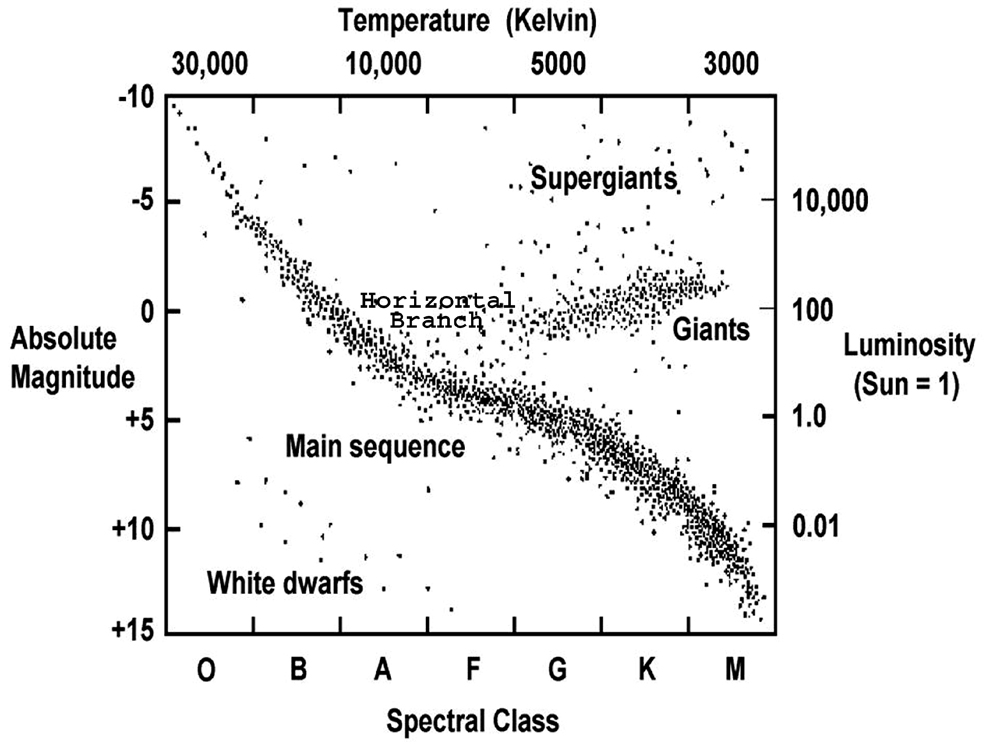
\includegraphics[scale=0.3]{HR_diagram.jpg}
        \\
        Hertzsprung-Russelův diagram\footnotemark[4]
    \end{center}
\end{figure}
\footnotetext[1]{Je potřeba vnímat dvě odslišné veličiny; jasnost a zářivost/svítivost.}
\footnotetext[2]{Česky by se správně mělo psát: Stefan\underline{ův}-Boltzmanův zákon – to nám však přijde opravdu uširvoucí.}
\footnotetext[3]{Existuje mnoho vtipných pořekadel na zapomatování si všech tříd. Doporučujeme vám si je najít. }
\footnotetext[4]{Ilustrace od Chandra X-ray Observatory edu, NASA}
logaritmicka mira (bud magnituda nebo HRD)
\\
\\
\textbf{Úloha:}

Proč nevidíme zelené nebo třeba fialové hvězdy?
\\
Při pohledu na HR diagram vás možná zaskočilo, že jeden dílek  stupnice zářivého výkonu (luminosity) neodpovída  jednomu dílku stupnice absolutní magnitudy.
%<*task>

%\begin{enumerate}[\noindent {}]
%\item otazka
%  \begin{choices}
%    \choice
%  \end{choices}
%\end{enumerate}

%</task>
\end{document}
